\chapter{Durchführung}
In diesem Kapitel wird auf die Durchführung der Messungen mit dem Passivradar eingegangen. Dabei wird erläutert werden, wo sich die Quelle des verwendeten Signals befindet und wo sich der Messpunkt befindet und nach welchen Kriterien er ausgewählt wurde. Außerdem wird der gesamte fertige Messaufbau dargestellt.
\section{Punkt des Signals}
Als Beleuchter dient der Stuttgarter Fernsehturm. Dieser liegt im Süden von Stuttgart und ist in Abbildung~\ref{fig:Fernsehturm} zu sehen. Das 5G Broadcast-Signal wird vom Stuttgarter Fernsehturm in Richtung der A8 ausgesendet. Der Broadcast ist Teil eines Pilotprojektes, gefördert durch einem Zusammenschluss aus Südwestrundfunk (SWR), Kathrein Broadcast GmbH,  DFMG  Deutsche Funkturm GmbH, Porsche AG, Rohde \& Schwarz GmbH \& Co. KG, TU Braunschweig und Telekom Deutschland GmbH benutzt. Das Ziel des Projektes ist es die Nutzung von 5G Broadcast für Anwendungen in Fahrzeugen zu erproben. Dafür werden vier Services übertragen: Zwei Fernsehprogramme, die ARD/SWR Mediathek und ein Reiseführer~\cite{5GMAG2020}.
\begin{figure}
    \centering
    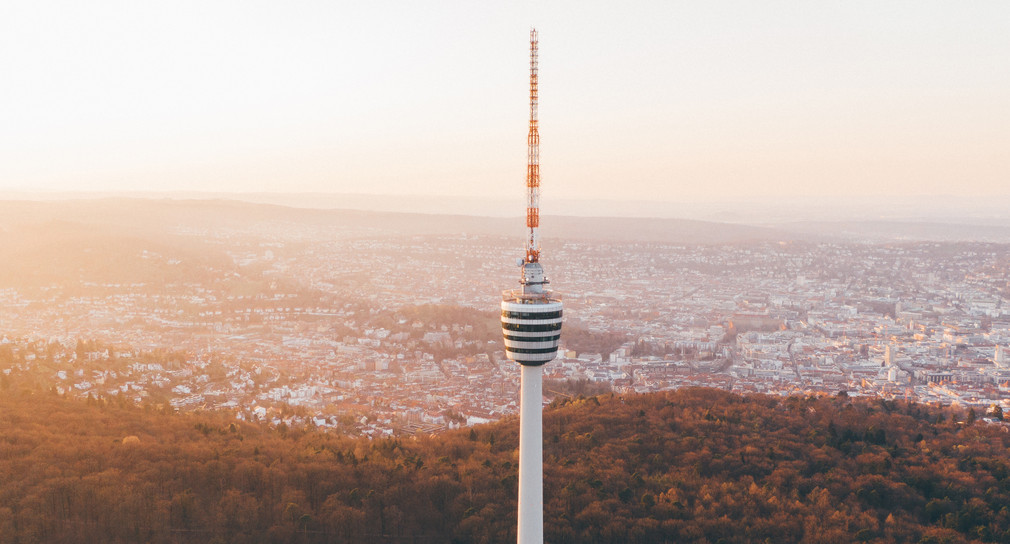
\includegraphics[width=\textwidth]{images/Fernsehturm.jpg}
    \quelle{\cite{TURM2021}}
    \caption{Stuttgarter Fernsehturm}\label{fig:Fernsehturm}
\end{figure}

\section{Messpunkt}
Der Ort der Feldmessungen ist so gewählt, dass sowohl der Stuttgarter Flughafen, als auch der Stuttgarter Fernsehturm für das Radar sichtbar sind. Da der Aufbau nicht im zusammengebauten Zustand transportfähig ist, muss dieser vor Ort montiert werden. Dies kann wertvolle Zeit kosten, weshalb der Messplatz bewusst in der Nähe des Studentenwohnheims Geschwister-Scholl-Str.\@ gewählt wurde. Unweit des Messplatzes befindet sich der Segelflugplatz Esslingen, jedoch konnten während den Feldmessungen keine Segelflugstarts oder Landungen beobachtet werden. Der Messaufbau wurde daher \SI{300}{\metre} südlich mit Blick auf das Tal verlegt. Die genaue Position ist in Abbildung~\ref{fig:Einflugschneise} und in Abbildung~\ref{fig:Maps} auf Google Maps zu erkennen.

\begin{figure}
    \centering
    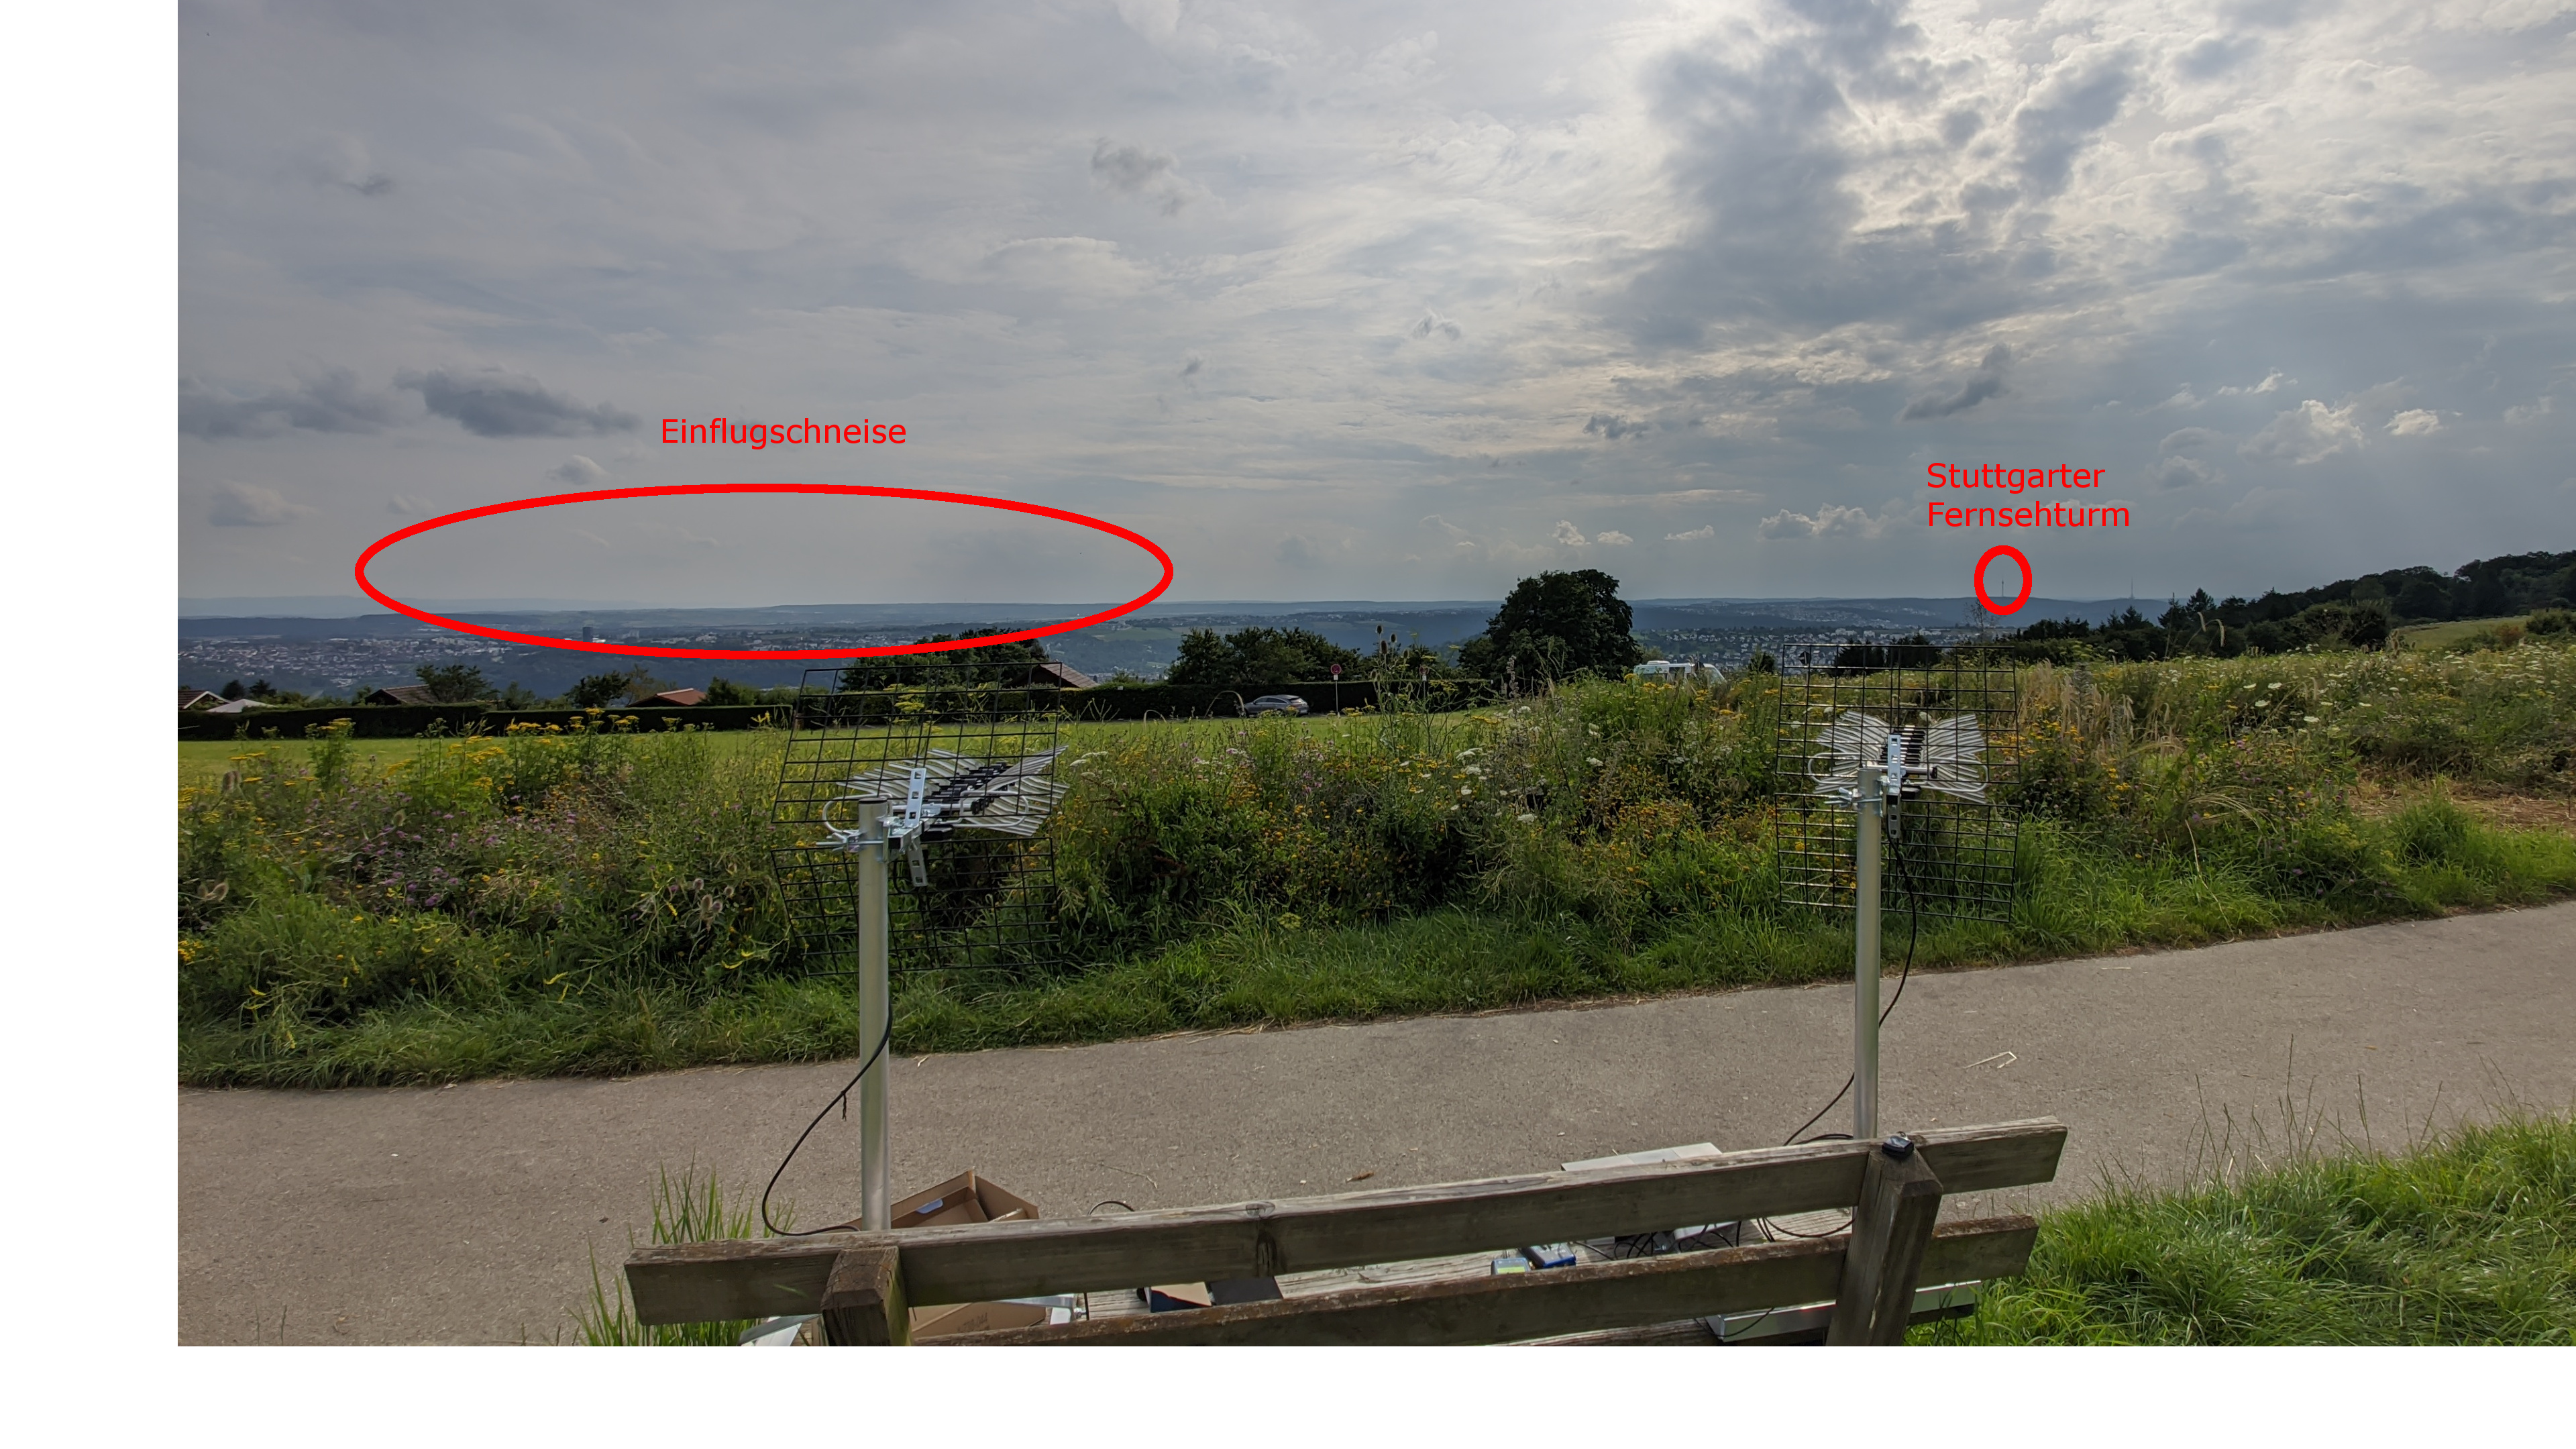
\includegraphics[width=\textwidth]{images/Einflugschneise.jpg}
    \caption{Einflugschneise und Stuttgart Fernsehturm}\label{fig:Einflugschneise}
\end{figure}

\begin{figure}
    \centering
    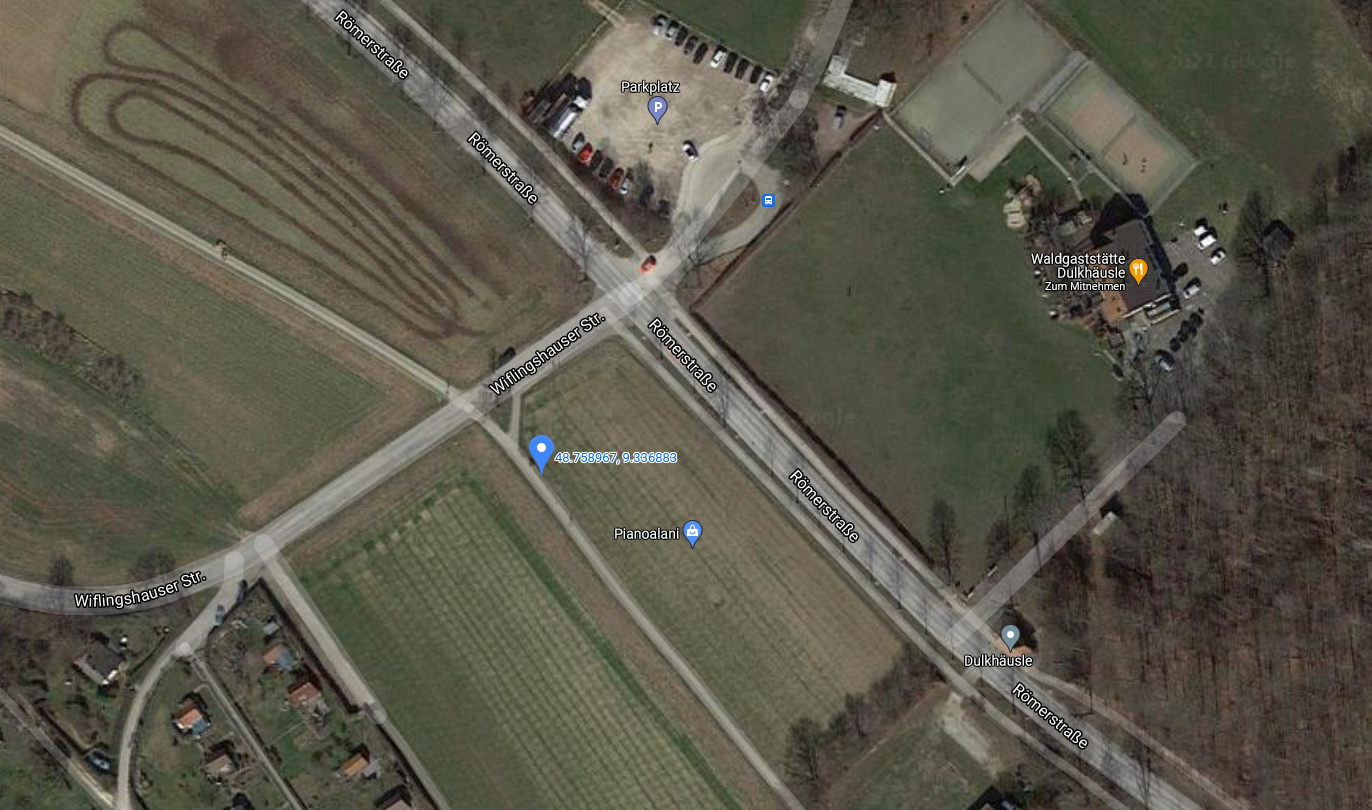
\includegraphics[width=\textwidth]{images/Maps_Messpunkt.png}
    \caption{Possition des Messpunkt}\label{fig:Maps}
\end{figure}

\section{Messaufbau}
Der Messaufbau besteht aus den Komponenten die im Kapitel~\ref{sct:setup} auf S.\pageref{sct:setup} erläutert wurden. Der gesamte fertige Aufbau ist dann in Abbildung~\ref{fig:Messaufbau} zu sehen hier werden die beiden SDRs~\ref{sct:sdr} sowie der OCXO Oscillator~\ref{sct:Oscillator} mit einem Laptop mit SDR-angel Sofware verbunden. Die Antennen sind so ausgerichtet, dass eine auf den Stuttgarter Flughafen ausgerichtet ist und die andere auf den Stuttgarter Fernsehturm, wie auch in Abbildung~\ref{fig:Einflugschneise} abgebildet.

\begin{figure}
    \centering
    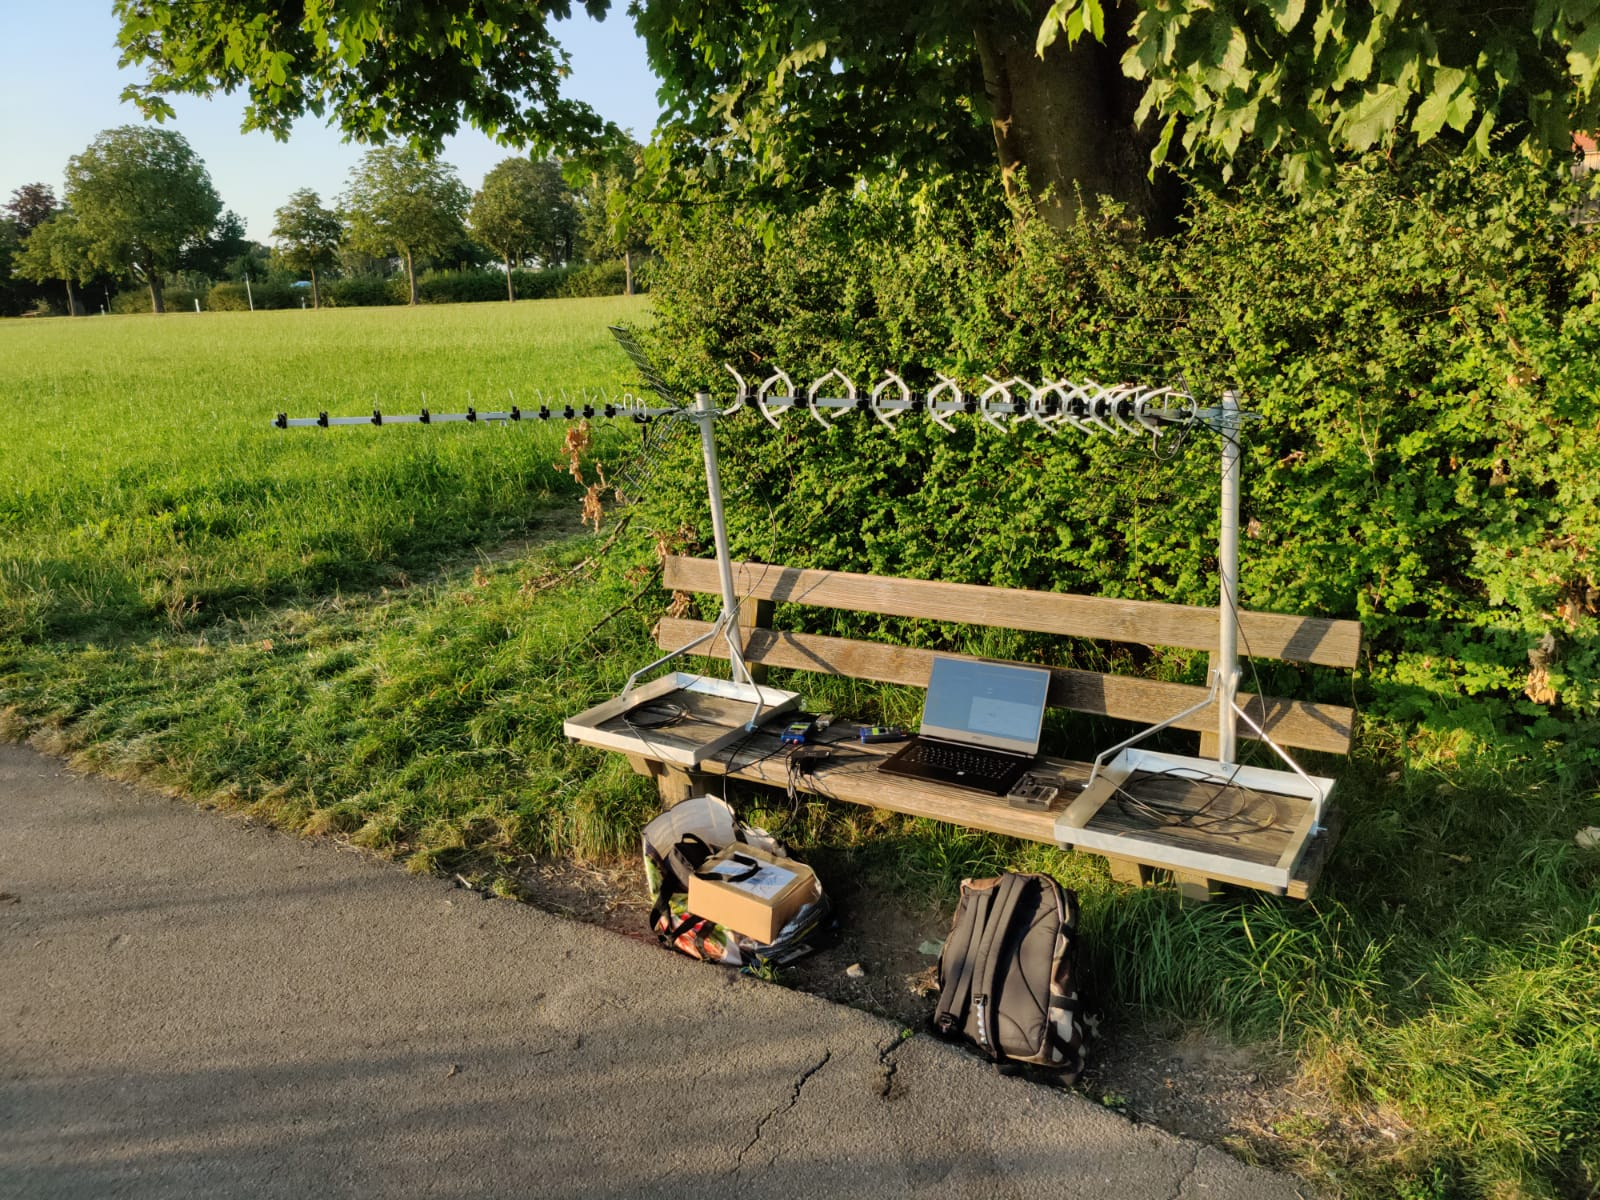
\includegraphics[width=\textwidth]{images/Messaufbau.jpg}
    \caption{Aufbau der Messung}\label{fig:Messaufbau}
\end{figure}
